% \documentclass[aspectratio=169]{beamer}
% \mode<presentation>

\documentclass[aspectratio=169,handout]{beamer}
\mode<presentation>
\setbeameroption{show notes}
\usepackage{pgfpages}
\pgfpagesuselayout{6 on 1}[letterpaper,border shrink=5mm]


%Theme and Color of Presentation
\usetheme{CambridgeUS}
\usecolortheme{seahorse}
\useinnertheme{rectangles}

%Colors
% From https://www.utdallas.edu/brand/color-palette/
\definecolor{UTDorange}{RGB}{232,117,0}
\definecolor{UTDgreen}{RGB}{18,71,52}
\definecolor{UTDseafoam}{RGB}{95,244,183}

\setbeamercolor{palette primary}{bg=UTDorange,fg=white}
\setbeamercolor{palette secondary}{bg=UTDgreen,fg=white}
\setbeamercolor{palette tertiary}{bg=UTDorange,fg=white}
\setbeamercolor{palette quaternary}{bg=UTDorange,fg=white}
\setbeamercolor{frametitle}{fg=UTDgreen}
\setbeamercolor{structure}{fg=UTDgreen} % itemize, enumerate, etc
\setbeamercolor{subsection in head/foot}{bg=UTDgreen,fg=white}


%Additional Packages
\usepackage{graphicx}
\usepackage{physics}
\usepackage{amsmath}
\usepackage{setspace}
\usepackage{textpos}
\usepackage{hyperref}
\usepackage{xcolor}

%Additional Settings/Commands
\newcommand{\extraspace}{\vskip 0.5em}

\AtBeginSection[]
{
	\begin{frame}
		\frametitle{Outline}
		\tableofcontents[currentsection]
	\end{frame}
}
%\AtBeginSubsection[]
%{
%	\begin{frame}
%		\frametitle{Outline}
%		\tableofcontents[currentsection,currentsubsection]
%	\end{frame}
%}

%Presentation Info
\title[2nd-order System Dynamics]{Introduction to 2\textsuperscript{nd}-order System Response}
% \subtitle{Forced Step-Response, Transfer Functions, and }
\author{Jonas Wagner}
\institute[UTDallas]{The University of Texas at Dallas}
% \date[ME GTF Interview - Fall 2021]{Mechanical Engineering Graduate Teaching Fellowship Teaching Example - Fall 2021}
% Updated since original usage
\date{}

\begin{document}
	
\begin{frame}
	\titlepage
\end{frame}

\addtobeamertemplate{frametitle}{}{%
	\begin{textblock*}{100mm}(.85\textwidth,-1cm)
		
\includegraphics[height=1cm]{Images/UT_Dallas_Logo}
	\end{textblock*}
}

\begin{frame}{Outline}
	\tableofcontents
	\note{
		TODO: include 4th-wall break notes
		\begin{itemize}
			\item Focus in this lecture demonstration will be on the process/math to demonstrate how/why a dynamical system's characteristic polynomial is crucial to the response of the system
			\item In a larger course, the motivation of these dynamics will be explored a lot more eariler on and we'd move into getting the intuitive understanding with applied examples after this lecture
			\item In this lecture itself, the motivation and system differential equation derivation will be brought up primarily as a refresher/review before jumping into applying the Laplace method to the example 2nd order system
			\item 
		\end{itemize}
	}
\end{frame}

\section{Background}
\begin{frame}
	\frametitle{Motivation: Real-World Dynamical System}
	
	TODO: add examples of dynamical systems

\end{frame}



\begin{frame}
	\frametitle{Review: Spring Mass-Damper System Model}
	\begin{columns}
		\begin{column}{0.5 \textwidth}
			Newton's 2\textsuperscript{nd} Law:
			\[
				F = m \vb{a} 
				= m \dv{t} \vb{v} 
				= m \dv{t} \qty(\dv{t} \vb{x})
			\]
			\[
				m \dv{t^2} x(t) 
				= \sum F 
				= f(t) - b \dv{t} x(t) - k x(t)
			\] 
			% \[
			% 	m \dv{t^2} x(t) + b \dv{t} x(t) + k \dv{t} x(t) = f(t)
			% \]
			\vspace{1em}

			Differential Equation: ($\vb{x} = x(t)$, $\vb{u} = f(t)$)
			% Let $\vb{x} = x(t)$ and $\vb{u} = f(t)$
			\[
				m \ddot{\vb{x}} + c \dot{\vb{x}} + k \vb{x} = \vb{u}
			\]
			
			% Let $\vb{x} = x(t)$ and $\vb{u} = f(t)$
			% \[
			% 	m \ddot{\vb{x}} + c \dot{\vb{x}} + k \vb{x} = \vb{u}
			% \]
			% \[
			% 	\ddot{\vb{x}} 
			% 	= \qty(\frac{-c}{m}) \dot{\vb{x}} + \qty(\frac{-k}{m}) \vb{x} + \qty(\cfrac{1}{m}) \vb{u}
			% \]
			% \[
			% 	\dv{t} \mqty[
			% 		\dot{\vb{x}}\\ 
			% 		\vb{x}
			% 	 ] = 
			% 	\mqty[
			% 		1 &0\\
			% 		-\frac{c}{m} &-\frac{k}{m}
			% 		] 
			% 	\mqty[
			% 		\dot{\vb{x}}\\
			% 		\vb{x}
			% 	]
			% 	+ \mqty[
			% 		0\\
			% 		\frac{1}{m}
			% 	]
			% 	\mqty[\vb{u}]
			% \]
		\end{column}
		\begin{column}{0.375 \textwidth}
			\begin{figure}[]
				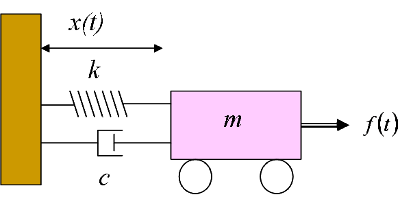
\includegraphics[width=\textwidth]{Images/SpringMassDamper_cartSystem.png}
				Spring Mass Damper System \cite{ctms_engin_umich_SystemModeling}
			\end{figure}
		\end{column}
	\end{columns}
\end{frame}



\section{Derivation: Laplace method to derive Step-Response}
\begin{frame}
	\frametitle{Spring-mass-damper Differential Equation:}
	\begin{align*}
		m \ddot{x}(t) + b \dot{x}(t) + k x(t) &= f(t)\\
		&\Downarrow \mathcal{L}\\
		m s^2 X(s) + b s X(s) + k X(s) &= F(s)\\
		(m s^2 + bs + k) X(s) &= F(s)
	\end{align*}
	\[
		X(s) = \frac{1}{ms^2 + b s + k} F(s)
	\]

	\textbf{Step Response:}
	$f(t) = u(t) \overset{\mathcal{L}}{\Rightarrow} F(s) = \frac{1}{s}$
	\[
		X(s) = \frac{1}{ms^2 + b s + k} \qty(\frac{1}{s})
		= \frac{1}{s(m s^2 + b s + k)}
		= \frac{\frac{1}{m}}{s (s^2 + \frac{b}{m}s + \frac{k}{m})}
	\]
		
	\note{
		Call the denomenator the characteristic polynomial, and demonstrate importnace when doing the partial fraction decomposition

		Characteristic Polynomial :\[
			\Delta(s)
			= m s^2 + b s + k
			% \Rightarrow s^2 + \frac{b}{m} s + \frac{k}{m}
			% = s^2 + 2 \zeta \omega_0 s + \omega_0^2
		\]
	}
\end{frame}
\begin{frame}
	\frametitle{Factoring the characteristic polynomial}
	In order to do the partial fraction decomposition, it must be in factored form, thus factoring via the quadratic equation: $\Delta(s) = m s^2 + b s + k$
	\begin{align*}
		s = \cfrac{-b \pm \sqrt{b^2 - 4mk}}{2m}
		= -\frac{b}{2m} \pm \sqrt{\frac{b^2 -4mk}{4m^2}}
		= -\frac{b}{2m} \pm \sqrt{\qty(\frac{b}{2m})^2 - \sqrt{\frac{k}{m}}^2}
	\end{align*}
	\note{This is equivalent to $\Delta(s) = s^2 + \frac{b}{m}s + \frac{k}{m}$\\}

	\textbf{3 Potential cases:} %(may have learned in differential equations)
	\begin{enumerate}
		\item \textbf{Damped}: $(\frac{b}{2m})^2 > \frac{k}{m} \Rightarrow (s+a)(s+b)$
		\item \textbf{Critically Damped}:$(\frac{b}{2m})^2 = \frac{k}{m} \Rightarrow (s + a)^2$
		\item \textbf{Underdamped}: $(\frac{b}{2m})^2 < \frac{k}{m} \Rightarrow (s + \sigma \pm j \omega)$
	\end{enumerate}
	
	\note{
	This motivates the standard characteristic polynomial form:
	\begin{align*}
		s^2 + 2 \zeta \omega_0 s + \omega_0^2
		\Rightarrow
		s = \zeta \omega_0 \pm \sqrt{(\zeta \omega_0)^2 - \omega_0^2}
		= \omega_0 \qty(\zeta \pm \sqrt{\zeta - 1})\\
		\intertext{Let $2 \zeta \omega_n = \sqrt{\frac{b}{m}}$ and $\omega_0 = \sqrt{\frac{k}{m}}$}
		\Delta(s) = s^2 + \frac{b}{m} s + \qty(\sqrt{\frac{k}{m}})^2
		\iff \Delta(s) = s^2 + 2\zeta \omega_0 s + \omega_0^2
	\end{align*}
	In this instance, the three cases are easily seen based on $\zeta$:
	\begin{enumerate}
		\item Damped: $\zeta > 1$
		\item Critically Damped: $\zeta = 1$
		\item Underdamped: $\zeta \in [0,1)$
	\end{enumerate}
	}
\end{frame}
\begin{frame}
	\frametitle{Case 1 (Damped)}
	Let $a = \frac{b}{2m} + \sqrt{\qty(\frac{b}{2m})^2 - \qty(\sqrt{\frac{k}{m}})^2}$ and $b = \frac{b}{2m} - \sqrt{\qty(\frac{b}{2m})^2 - \qty(\sqrt{\frac{k}{m}})^2}$
	\begin{gather*}
		X(s) 
		= \cfrac{1}{m s (s^2 + \frac{b}{m}s + \frac{k}{m})}
		= \cfrac{\frac{1}{m}}{s(s+a)(s+b)}
		\intertext{
			Evaluate Coefficients:
			$C_{i} = \eval{\frac{(s-\lambda_{i})}{m (s(s+a)(s+b))}}_{s = \lambda_{i}}$
		}
		X(s) = \cfrac{C_1}{s} + \cfrac{C_2}{s+a} + \cfrac{C_3}{s+b}
		\overset{\mathcal{L}}{\iff}
		x(t) = \qty(C_1 + C_2 e^{-at} + C_3 e^{-bt}) u(t)
	\end{gather*}

	\note{
		% \[
		% 	C_{1,2,3} = \eval{\cfrac{\frac{1}{m}}{s(s+a)(s+b)}(s-\lambda_{i})}_{s = \lambda_{i}}
		% \]
		Evaluate coeficients:
		$(a)(b) = (\frac{b}{2m})^2 - ((\frac{b}{m})^2-\frac{k}{m}) = \frac{k}{m}$, \quad $(a-b) = 2\sqrt{(\qty(\frac{b}{2m})^2 - \frac{k}{m})}$
		\begin{gather*}
			C_1 = \eval{\frac{(s)}{m s(s+a)(s+b)}}_{s=0}
			= \frac{1}{m (a)(b)}
			\Rightarrow
			C_1 = \frac{1}{k} \textbf{(Hook's Law @ steady-state)}
			\\
			C_2 = \eval{\frac{(s+a)}{m s(s+a)(s+b)}}_{s=-a}
			= \frac{1}{m(-a)(-a+b)}
			= \frac{1}{m(a)(a-b)}
			\\
			C_3 = \eval{\frac{(s+b)}{m s(s+a)(s+b)}}_{s=-b}
			= \frac{1}{m(-b)(a-b)}
			= \frac{-1}{m(b)(a-b)}\\
			C_{2,3} = \cfrac{\pm 1}{2m\sqrt{(\qty(\frac{b}{2m})^2 - \frac{k}{m})} \qty(\frac{b}{2m} \pm \sqrt{\qty(\frac{b}{2m})^2 - \qty(\sqrt{\frac{k}{m}})^2})}
		\end{gather*}
	}
	
\end{frame}

\begin{frame}
	\frametitle{Case 2 (Critically Damped)}
	Let $a = \frac{b}{2m}$
	\begin{gather*}
		X(s) = \cfrac{\frac{1}{m}}{s (s+a)^2} 
		= \cfrac{C_1}{s} + \cfrac{C_2}{s+a} + \cfrac{C_3}{(s+a)^2}
		\overset{\mathcal{L}}{\Rightarrow}
		x(t) = \qty(C_1 + C_2 e^{-a t} + C_3 t e^{-a t}) u(t)
	\end{gather*}
\end{frame}

\begin{frame}
	\frametitle{Case 3 (Underdamped)}
	Let $\sigma = \frac{b}{m}$ and $\omega = \sqrt{\sqrt{\frac{k}{m}}^2 - \qty(\frac{b}{2m})^2}$
	
	\begin{align*}
		X(s) &= \cfrac{\frac{1}{m}}{s (s+\sigma \pm j\omega)} 
		= \cfrac{C_1}{s} + \cfrac{C_2}{(s+\sigma+j\omega)} + \cfrac{C_3}{(s+\sigma - j\omega)}\\
		& \qquad \Updownarrow \mathcal{L}\\
		% \overset{\mathcal{L}}{\Rightarrow}\\
		% \overset{\mathcal{L}}{\Rightarrow}
		x(t) &= \qty(C_1 + C_2 e^{-\sigma t}e^{j\omega t} + C_3 e^{-\sigma t} e^{-j\omega t}) u(t)\\
		&= C_1 u(t) + 2 e^{-\sigma t} u(t) \frac{C_2 e^{j\omega t} + C_3 e^{-j\omega t}}{2}
		\Leftarrow \textbf{Convert using Euler's Identity}
	\end{align*}
	

\note{
	Alternative approach
	\begin{align*}
		X(s) &= \cfrac{\frac{1}{m}}{s (s^2 + \frac{b}{m}s + \frac{k}{m})}
		= \cfrac{C_1}{s} + \cfrac{C_2}{(s+\frac{b}{2m})^2 + \sqrt{\frac{k}{m}-\sqrt{\frac{b}{m}}}^2}
		\overset{\mathcal{L}}{\Rightarrow}\\
		&\overset{\mathcal{L}}{\Rightarrow}
		x(t) = \qty(C_1 + \frac{C_2}{\sqrt{\frac{k}{m}-\sqrt{\frac{b}{m}}}} \exp{-\cfrac{b}{2m}t} \cos{\qty(\sqrt{\frac{k}{m}-\sqrt{\frac{b}{m}}})t}) u(t)
	\end{align*}
}

\end{frame}
% \note{	
% 	Characteristic Polynomial :\[
% 		\Delta(s)
% 		= m s^2 + b s + k
% 		\Rightarrow s^2 + \frac{b}{m} s + \frac{k}{m}
% 		% = s^2 + 2 \zeta \omega_0 s + \omega_0^2
% 	\]
% }



	
	% 2\textsuperscript{nd}-Order Dynamical System:
	% \[
	% 	\ddot{x}(t) + 2 \zeta \omega_0 \dot{x}(t) + \omega_0^2 x(t) = u(t)
	% \]


% \note{

% \begin{align*}
% 	m \ddot{x}(t) + b \dot{x}(t) + k x(t) &= f(t)\\
% 	&\Downarrow \mathcal{L}\\
% 	m s^2 X(s) + b s X(s) + k X(s) &= F(s)\\
% 	(m s^2 + bs + k) X(s) &= F(s)\\
% 	X(s) &= \frac{1}{ms^2 + b s + k} F(s)
% 	% s^2 X(s) + \frac{b}{m} s X(s) + \frac{k}{m} X(s) &= \frac{1}{m} F(s)\\
% 	% \qty(s^2 + \frac{b}{m} s + \frac{k}{m}) X(s) &= \frac{1}{m} F(s)\\
% 	% X(s) &= \cfrac{\frac{1}{m}}{s^2 + \frac{b}{m} s + \frac{k}{m}} F(s)\\
% 	% TODO: factor it here...
% \end{align*}
% Charectoristic Polynomial :\[
% 	\Delta(s)
% 	= m s^2 + b s + k
% 	\Rightarrow s^2 + \frac{b}{m} s + \frac{k}{m}
% 	= s^2 + 2 \zeta \omega_0 s + \omega_0^2
% \]

% } \note{

% In order to do the partial fraction decomposition, it must be in factored form... 
% thus the quadratic equation:
% \[
% 	\Delta(s) = m s^2 + b s + k = 0 
% 	\Rightarrow s 
% 	= \cfrac{-b \pm \sqrt{b^2 - 4mk}}{2m}
% 	= \frac{b}{2m} \pm \sqrt{\frac{b^2 -4mk}{4m^2}}
% 	= \frac{b}{2m} \pm \sqrt{\qty(\frac{b}{2m})^2 - \frac{k}{m}}
% \]

% 3 Potential cases: (may have learned in differential equations)
% \begin{enumerate}
% 	\item \textbf{Damped}: $(\frac{b}{2m})^2 > \frac{k}{m} \Rightarrow (s+a)(s+b)$
% 	\item \textbf{Critically Damped}:$(\frac{b}{2m})^2 = \frac{k}{m} \Rightarrow (s + a)^2$
% 	\item \textbf{Underdamped}: $(\frac{b}{2m})^2 < \frac{k}{m} \Rightarrow (s + \sigma \pm j \omega_d)$
% \end{enumerate}

% We will continue under the assumption that the system is underdamped and then return for a more general case.

% } 
% \note{

% Step Response: 
% $f(t) = u(t) \overset{\mathcal{L}}{\Rightarrow} F(s) = \frac{1}{s}$
% \begin{align*}
% 	X(s) 
% 	&= \cfrac{\frac{1}{m}}{s^2 + \frac{b}{m} s + \frac{k}{m}} \qty(\frac{1}{s})
% 	= \cfrac{\frac{1}{m}}{s(s^2 + \frac{b}{m} s + \frac{k}{m})}
% 	\\
% 	\intertext{
% 		Factored Form (quadratic formula):
% 	$a s^2 + b s + c = 0 \Rightarrow s = \cfrac{-b \pm \sqrt{b^2 - 4ac}}{2a}$
% 	}
% 	TODO: factor it... 3 cases...
% 	% X(s) &= \cfrac{\frac{1}{m}}{s (s + \cfrac{\frac{b}{m} \pm \sqrt{(\frac{b}{m})^2 - 4 \frac{k}{m}}}{2})}\\
% 	\intertext{Partial Fraction Expansion}
% 	X(s) &= 
% \end{align*}

% } \note{	

% Side Note: (skip unless time allows/go back to this)
% Looking at the original differential equation we can see how the standard form $s^2 + 2\zeta \omega_0 s + (\omega_0)^2$ would fit in as \[
% 	\zeta \omega_0 \pm \sqrt{(\zeta \omega_0)^2 - \omega_0^2}
% 	= \zeta \omega_0 \pm \sqrt{\omega_0^2 (\zeta^2 - 1)}
% 	= \zeta \omega_0 \pm \omega_0 \sqrt{\zeta^2 - 1}
% \]

% }










\begin{frame}
	\frametitle{TLDR: Second-Order System Dynamics}
	\begin{columns}
		\begin{column}{0.5\textwidth}
			\textbf{Transfer Function}
			\[
				H(s) 
				= \cfrac{Y(s)}{U(s)} 
				= \cfrac{
					\omega_0^2
				}{
					s^2 + 2 \zeta \omega_0 s + \omega_0^2
				}
			\]
			\textbf{System Poles}
			\[
				s = - \zeta \omega_0 \pm \omega_0 \sqrt{1 - \zeta^2}
			\]
			\textbf{Spring Mass Damper System Parameters}
			\[
				\omega_0 = \sqrt{\cfrac{k}{m}}
				\hspace{0.5 in}
				\zeta = \sqrt{\cfrac{c^2}{4 m k}}
			\]
		\end{column}
		\begin{column}{0.375\textwidth}
			\begin{figure}[]
				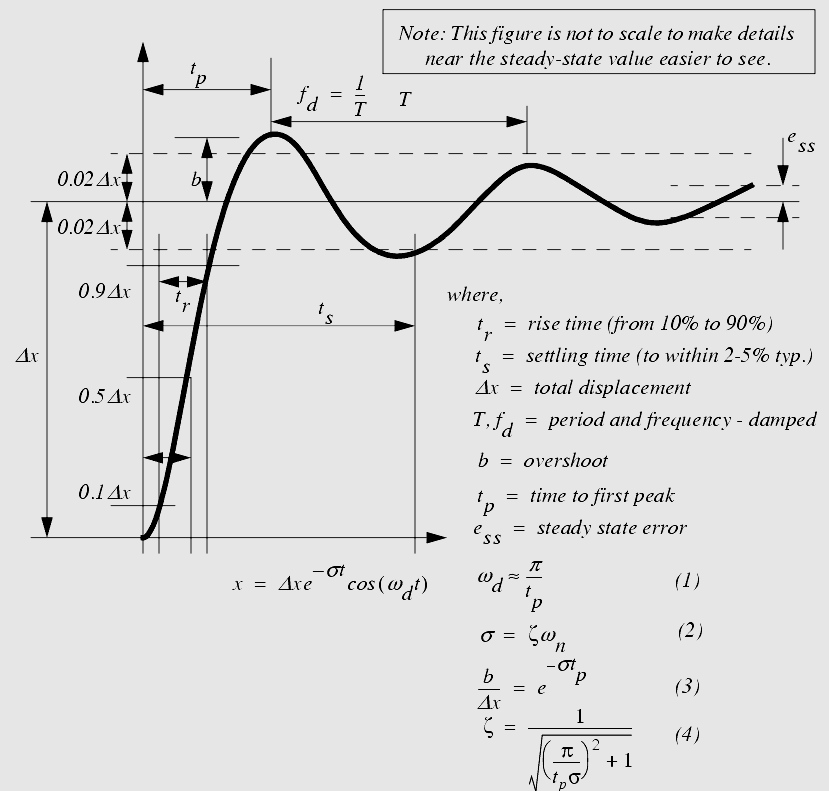
\includegraphics[width=\textwidth]{Images/2ndOrderTransient.png}
				2nd Order System Response \cite{engineerOnADisk_2ndOrderDynamics}
			\end{figure}
		\end{column}
	\end{columns}
\end{frame}

% \section{Steady-state Forced Response}
% \begin{frame}
% 	\frametitle{Review: Steady-state Input System Response}
% 	\begin{figure}
% 		\centering
% 		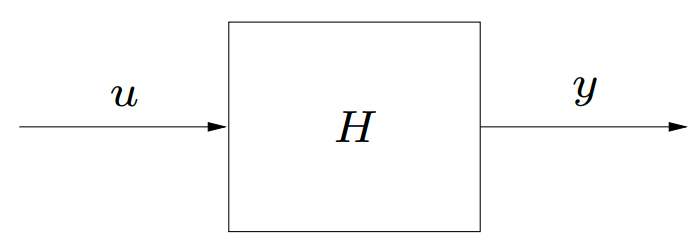
\includegraphics[width = 0.25\textwidth]{Images/H(s)_BlockDiagram.png}
% 	\end{figure}
% 	\textbf{Convolution:} 
% 	\[
% 		y(t) = \int_{0}^{t} h(\tau) u(t - \tau) \dd \tau 
% 		\quad 
% 		Y(s) = H(s) U(s)
% 	\]
% 	\textbf{Sinusoidal Input:} 
% 	\[
% 		u(t) = cos(\omega t) = (e^{j\omega t} + e^{-j\omega t})/2 = 1 e^{j 0}
% 	\]
% 	\textbf{Steady-State Output:} 
% 	\[
% 		y(t) = \int_{0}^{\infty} h(\tau) cos(\omega (t - \tau)) \dd \tau = A e^{j \phi} = A \cos(\omega t + \phi)
% 	\]
% 	where $A = \abs{H(j \omega)}$ and $\phi = \angle(H(j \omega))$.
% \end{frame}


% \begin{frame}
% 	\frametitle{Steady-state System Response}
% 	\begin{columns}
% 		\begin{column}{0.3\textwidth}
% 			\textbf{Magnitude Gain:} 
% 			\[\abs{H(j\omega)} = \frac{Y_0}{U_0} = \frac{1.5}{2} = 0.75\]
% 			\textbf{Phase Shift:}
% 			\[\angle{H(j\omega)} = \phi = \frac{\pi}{4}\]
% 		\end{column}
% 		\begin{column}{0.5\textwidth}
% 			\[
% 				\color{red}
% 				u(t) = U_0 \cos(\omega t)
% 				\quad
% 				\color{blue}
% 				y(t) = Y_0 \cos(\omega t + \phi)
% 			\]
% 			\begin{figure}
% 				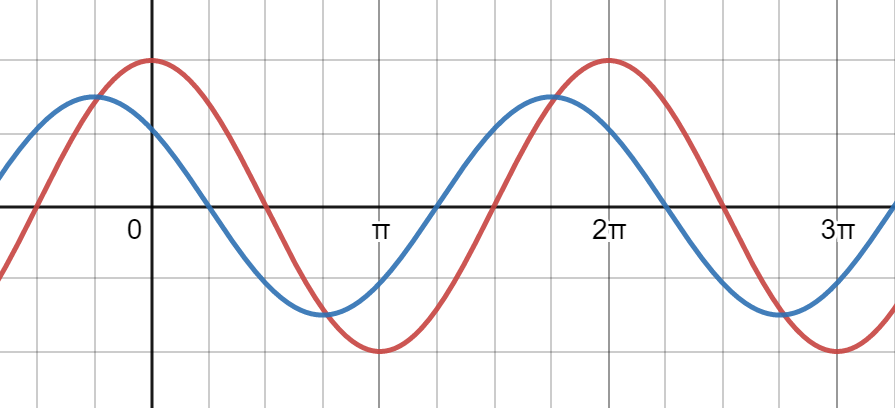
\includegraphics[width=\textwidth]{Images/phase_shift.png}
% 				Steady-state System Response with $\omega = 1$.
% 			\end{figure}
% 			\footnotesize{
% 				\textbf{Homework 6:}
% 				Sketch Bode Plots for given Transfer Functions
% 				\tiny{See posted review lectures for examples}
% 			}
% 		\end{column}
% 	\end{columns}
% 	\note{
% 		It is important to 
% 	}
% \end{frame}

% \section{Frequency Dependent Forced Response}
% \begin{frame}
% 	\frametitle{Activity: Spring Mass Damper Frequency Response
% 	\cite{swarthmore_freq_response}}
% 	\begin{figure}
% 		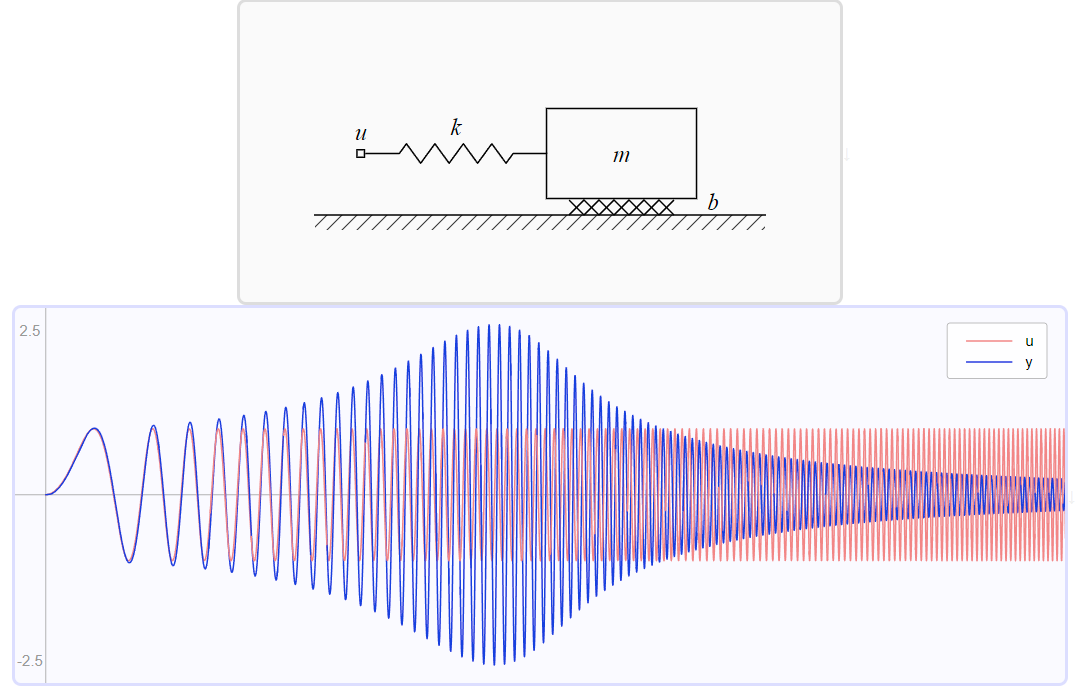
\includegraphics[width=0.625\textwidth]{Images/visualize_varied_freq_response.png}
% 		https://www.sccs.swarthmore.edu/users/12/abiele1/Linear/examples/freq.html
% 	\end{figure}
% \end{frame}

% \begin{frame}
% 	\frametitle{Bode Plot}
% 	\begin{columns}
% 		\begin{column}{0.375\textwidth}
% 			\textbf{Transfer Function:}
% 			\[
% 				H(s) 
% 				% = \cfrac{Y(s)}{U(s)} 
% 				= \cfrac{
% 					\omega_0^2
% 				}{
% 					s^2 + 2 \zeta \omega_0 s + \omega_0^2
% 				}
% 			\]
% 			\textbf{Magnitude Gain:} 
% 			\[\abs{H(j\omega)}_{db} = 20 \log_{10} \abs{\frac{Y_0}{U_0}}\]
% 			\textbf{Phase Shift:}
% 			\[\angle{H(j\omega)} = \phi\]
% 		\end{column}
% 		\begin{column}{0.5\textwidth}
% 			\begin{figure}
% 				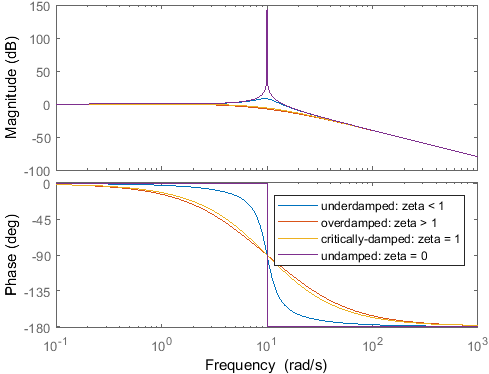
\includegraphics[width=\textwidth]{Images/bode_diagram.png}
% 				Bode Diagram varying dampening factor, $\zeta$.
% 			\end{figure}
% 		\end{column}
% 	\end{columns}
% \end{frame}	

% \begin{frame}
% 	\frametitle{Activity: Transfer Function Frequency Response}
% 	Investigate the system response by varying the input frequency, amplitude, and phase.
% 	{\cite{swarthmore_bode}}
% 	\begin{columns}
% 		\begin{column}{0.5\textwidth}
% 			\begin{figure}
% 				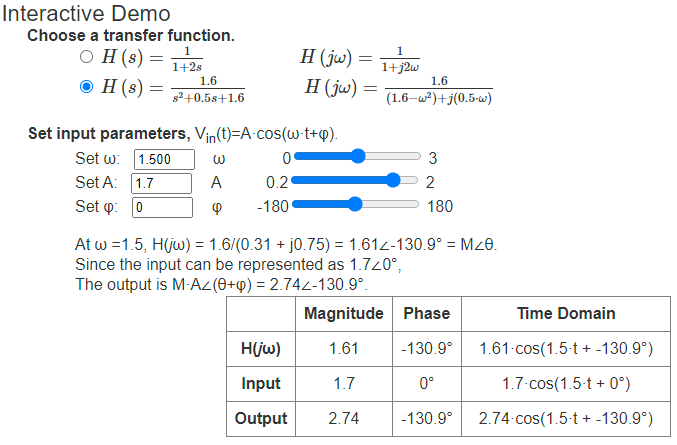
\includegraphics[width=\textwidth]{Images/bode_demo_1.png}
% 			\end{figure}
% 			\footnotesize{https://lpsa.swarthmore.edu/Bode/BodeWhat.html}
% 		\end{column}
% 		\begin{column}{0.4\textwidth}
% 			\begin{figure}
% 				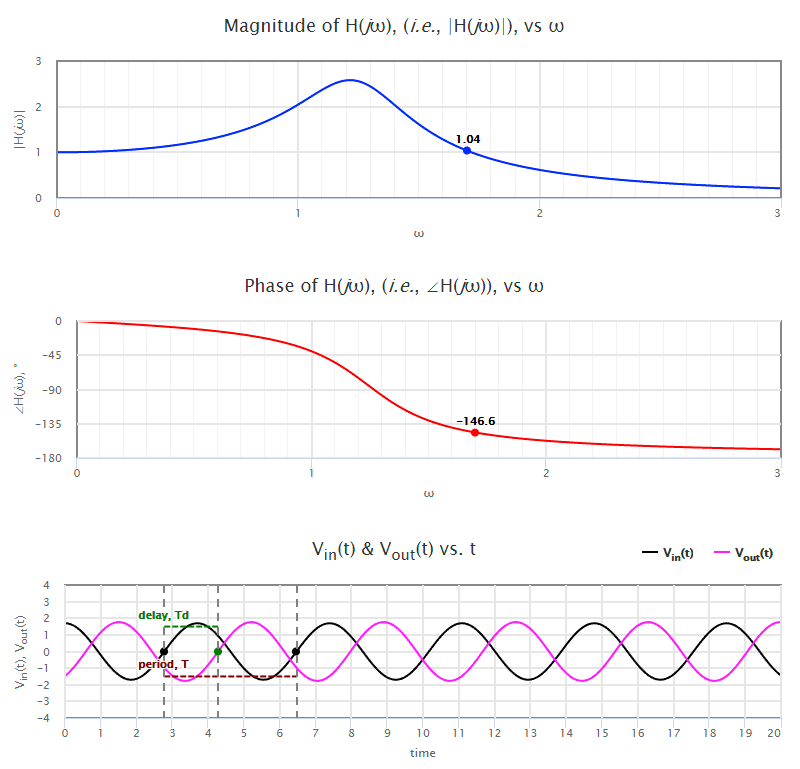
\includegraphics[width=\textwidth]{Images/bode_demo_2.png}
% 			\end{figure}
% 		\end{column}
% 	\end{columns}
% \end{frame}

% \section{Frequency Response System Characterization}
% \begin{frame}
% 	\frametitle{Real-World Applications: System Characterization}
% 	\begin{columns}
% 		\begin{column}{0.375\textwidth}
% 			\centering
% 			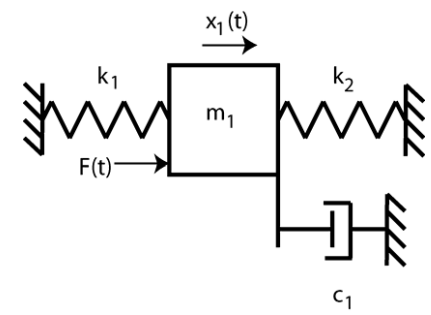
\includegraphics[width=0.75\textwidth]{Images/sys_char_diagram.png}\\
% 			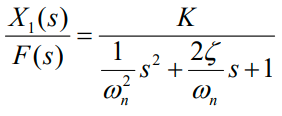
\includegraphics[width=0.5\textwidth]{Images/sys_char_tf.png}\\
% 			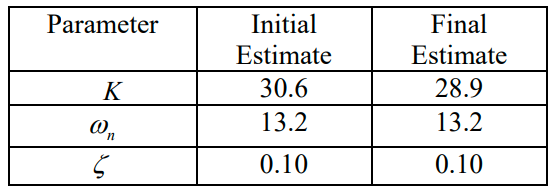
\includegraphics[width=\textwidth]{Images/sys_char_results.png}\\
% 			\footnotesize{System Characterization Paper Results 
% 			\cite{freq_response_charectorization}}
% 		\end{column}
% 		\begin{column}{0.5\textwidth}
% 			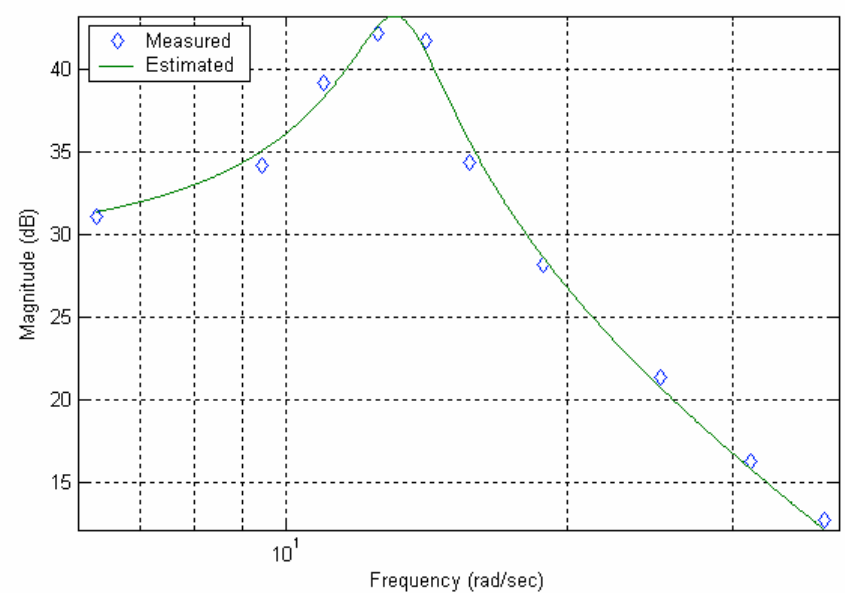
\includegraphics[width=\textwidth]{Images/sys_char_bode_data.png}
% 			\footnotesize{
% 				\textbf{Lab 3:}
% 				Experiment with selected system to obtain frequency response and characterize dynamics with an appropriate transfer function.
% 				\tiny{See lab instructions for more details}
% 				}
% 		\end{column}
% 	\end{columns}
% \end{frame}

\section*{}

\begin{frame}
	\frametitle{Lecture Overview}
	\begin{columns}
		\begin{column}{0.25\textwidth}
			\[
				m \ddot{x}(t) + b \dot{x}(t) + k x(t) = f(t)
				\quad \Rightarrow \quad
				\omega_0 = \sqrt{\frac{k}{m}}
				,
				\zeta = \sqrt{\frac{c^2}{4 m k}}
				,
				u(t) = \frac{1}{m} f(t)	
			\]
			\[
				H(s)
				= \frac{
					\omega_0^2
				}{
					s^2 + 2 \zeta \omega_0 s + \omega_0^2
				}
			\]
			\[
				\omega_0 = \sqrt{\frac{k}{m}}
				\quad
				\zeta = \sqrt{\frac{c^2}{4 m k}}
			\]
			\begin{figure}[]
				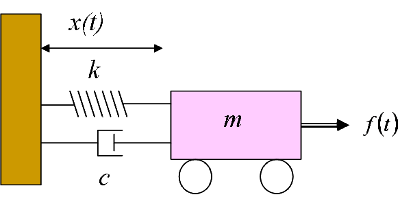
\includegraphics[width=\textwidth]{Images/SpringMassDamper_cartSystem.png}
			\end{figure}
		\end{column}
		% \begin{column}{0.3\textwidth}
		% 	\[
		% 		\color{red}
		% 		u(t) = U_0 \cos(\omega t)
		% 	\]
		% 	\[
		% 		\color{blue}
		% 		y(t) = Y_0 \cos(\omega t + \phi)
		% 	\]
		% 	\begin{figure}
		% 		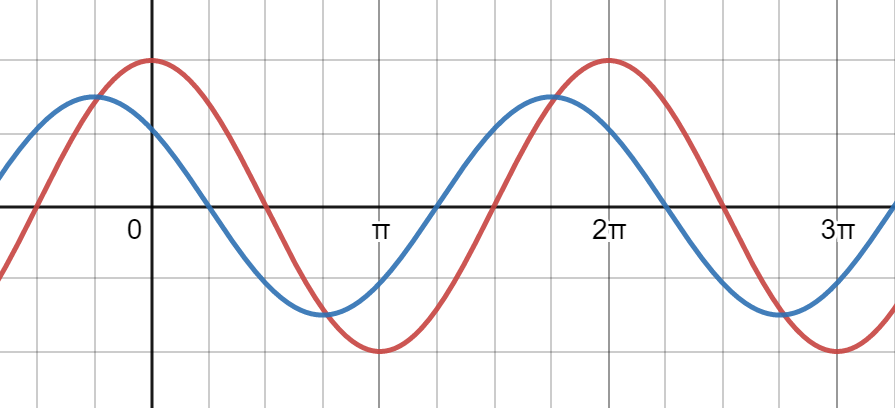
\includegraphics[width=\textwidth]{Images/phase_shift.png}
		% 	\end{figure}
		% \end{column}
		% \begin{column}{0.4\textwidth}
		% 	\begin{figure}
		% 		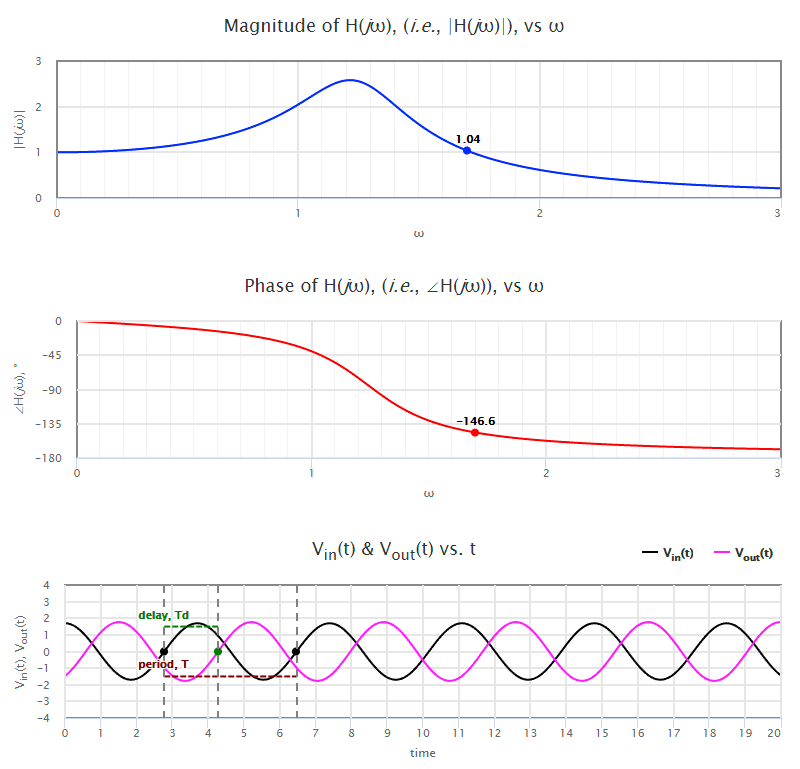
\includegraphics[width=\textwidth]{Images/bode_demo_2.png}
		% 	\end{figure}
		% \end{column}
	\end{columns}
\end{frame}

% \begin{frame}[allowframebreaks]{Bibliography}
% 	\bibliographystyle{unsrt}
% 	\bibliography{refs}
% \end{frame}


\end{document}